\section{Example}
\label{sec:example}
We next present major steps in our approach for detecting the behavioral differences of mapped API invocations. In particular, we use the \CodeIn{java.io.BufferedInputStream} class and the JLCA translation tool as illustrative examples.

\textbf{Translating generated wrapper methods.} As described by its documentation\footnote{\url{http://tinyurl.com/2bca7vh}}, the \CodeIn{BufferedInputStream} class in Java has 5 fields, 2 constructors, and 8 methods. To fully explore the behaviors of the class, TeMAPI generates a wrapper method for each field and method given each constructor. For example, given the \CodeIn{Buffered- InputStream(InputStream)} constructor, TeMAPI generates the wrapper method as follows for the \CodeIn{skip(long)} method:

\begin{CodeOut}\vspace*{-1ex}
\begin{alltt}
public long testskip24nm(long m0,InputStream c0)\{
  BufferedInputStream obj = new BufferedInputStream(c0);
  return obj.skip(m0);
\}  
\end{alltt}
\end{CodeOut}\vspace*{-2ex}

Each wrapper method check the return value of only one API method or field. If outputs are different given the same inputs, it is easy to locate the method or field with behavior differences and to find the inputs that cause behavior differences. TeMAPI next uses JLCA and translates generated wrapper from Java to C\#.

\textbf{Handling compilation errors.} In general, a translation tool may not include mapping relations for all API methods of a language. Therefore, translated wrapper methods can have compilation errors. TeMAPI parses translated wrapper methods and removes all wrapper methods with compilation errors. For example, following is the translated C\# \CodeIn{testskip24nm} method:

\begin{CodeOut}\vspace*{-1ex}
\begin{alltt}
public virtual long testskip24nm(long m0, Stream c0)\{
  BufferedStream obj = new BufferedStream(c0);
  BufferedStream temp_BufferedStream = obj;;
  Int64 temp_Int64 = temp_BufferedStream.Position;
  temp_Int64 = temp_BufferedStream.Seek(m0, 
        System.IO.SeekOrigin.Current) - temp_Int64;
  return temp_Int64;
\}
\end{alltt}
\end{CodeOut}\vspace*{-2ex}

TeMAPI does not removes this method since it has no compilation errors. Although JLCA translates the \CodeIn{skip(long)} method into multiple methods, we can still test the mapping relation since all translated code is within the wrapper method and a translation tool does not change the signatures of a wrapper method.  

\textbf{Generating test cases.} TeMAPI leverages various techniques to generate test cases for the remaining wrapper methods. For example, TeMAPI extends Pex~\cite{tillmann2008pex}, a state-of-the-art test generation technique, to record all inputs and their corresponding outputs generated for each translated wrapper method. Each input generated by Pex exercises a unique feasible path in the wrapper method. For example, TeMAPI generates the following JUnit test case based on inputs generated by Pex.

\begin{CodeOut}\vspace*{-1ex}
\begin{alltt}
public void testskip24nm36()\{
  try\{
     sketch.Test_java_io_BufferedInputStream obj = 
        new sketch.Test_java_io_BufferedInputStream();
     long m0 = java.lang.Long.valueOf(
                  "-9223372036582079488").longValue();
     InputStream c0 = new InputStream(null);
     obj.testskip24nm(m0,c0);
  \}catch(java.io.IOException e)\{
     Assert.assertTrue(true);return;
  \}
  Assert.assertTrue(false);
\}
\end{alltt}
\end{CodeOut}\vspace*{-2ex}

This test case fails, since given the preceding inputs, the \CodeIn{skip (long)} method does not throw any exceptions as the translated C\# code does. Thus TeMAPI detects a behavioral difference between the \CodeIn{skip(long)} method in Java and its mapped C\# API methods defined by JLCA.

Besides extending Pex, TeMAPI also extends Randoop~\cite{pacheco2007feedback} to generate invocation sequences. TeMAPI extracts the list of translated wrapper methods without compilation errors, and analyzes generated wrappers for a list of translatable API methods and fields. When generating test cases, TeMAPI limits the search scope of Randoop, so that each generate test case invoke only translatable API methods and fields. For example, a generated JUnit test case is as follows:

\begin{CodeOut}\vspace*{-1ex}
\begin{alltt}
public void test413() throws Throwable\{
  ...
  ByteArrayInputStream var2=new ByteArrayInputStream(...);
  var2.close();
  int var5=var2.available();
  assertTrue(var5 == 1);
\}
\end{alltt}
\end{CodeOut}\vspace*{-2ex}


TeMAPI next uses JLCA and translates the generated JUnit test case from Java to C\#. As each wrapper method invokes only translatable API invocations, we increase the chance of translating successfully. The translated NUnit test case is as follows:

\begin{CodeOut}\vspace*{-1ex}
\begin{alltt}
public void test413() throws Throwable\{
  ...
  MemoryStream var2 = new MemoryStream(...);
  var2.close();
  long available = var2.Length - var2.Position;
  int var5 = (int) available;
  UnitTool.assertTrue(var5 == 1);
\}
\end{alltt}
\end{CodeOut}\vspace*{-2ex}

The preceding JUnit test case gets passed, but the NUnit test case get failed. We find that Java allows programmers to access a stream even if the stream is closed, so the preceding JUnit test case run successfully. C\# does not allow such accesses, so the preceding NUnit test case fails with \CodeIn{ObjectDisposedException}. This example motivates our basic idea of generating test cases in one language and translating those test cases into another language for detecting differences among API mapping relations. We next present details of our approach.

%\begin{figure}[t]
%\centering %\hfill
%\includegraphics[scale=0.95,clip]{figure/sample.eps}\vspace*{-3ex}
% \caption{\label{fig:example}API mapping}\vspace*{-4ex}
%\end{figure}

%Based on the mapping relations, a translation tool can migrate the
%preceding code snippet automatically. To learn the mapping
%relations,
%
%%\begin{figure}[t]
%%\centering
%%\includegraphics[scale=0.86,clip]{figure/openfile.eps}\vspace*{-1.5ex}
%% \caption
%%{\label{fig:openfile}Aligned wrapper}\vspace*{-2ex}
%%\end{figure}
%
%In this section, we illustrate the main steps of MAM to
%mine the API mapping in Java for \CodeIn{System.IO.Directory.
%Exists()} in C\# from the HypoLog
%project\footnote{\url{http://sourceforge.net/projects/twlog/}}.
%
%The first step of MAM is to align classes and methods of
%wrapper by names. This step finds class pairs and method pairs
%that implement similar functionalities, and each pair may use
%API mapping since it implements a similar functionality. Our
%approach chooses names to align classes and methods because these
%classes and methods are from the same project. In this example, our
%approach aligns the two methods as shown in
%Figure~\ref{fig:openfile} because the two method have similar names
%and their declaring classes also have similar names (see
%Section~\ref{sec:approach:alignclientcode} for details).
%
%The second step of MAM is to mine mapping relations of API
%classes based on the names of corresponding fields, parameters,
%returned types, and local variables. This step also relies on names
%for the same consideration of the first step. For example, our
%approach maps the two parameters with the same name as shown by the
%red arrow of Figure~\ref{fig:openfile}. From the types of the two
%parameters, MAM mines the mapping relation between two API
%classes: \CodeIn{System.String} $\leftrightarrow$
%\CodeIn{java.lang.String} (see
%Section~\ref{sec:approach:mappingtypes} for details).
%
%
%The final step of MAM is to mine mapping relations of API
%methods. Besides the factors listed in
%Section~\ref{sec:introduction}, another factor is that API calls in
%wrapper are often not carefully aligned. To deal with those
%challenges, MAM first builds an API Transformation Graph
%(ATG) for each method. After that, MAM compares built
%graphs to mine mapping relations of API methods (see
%Section~\ref{sec:approach:mappingtypes} and
%Figure~\ref{fig:approach1} for details). Figure~\ref{fig:example}
%shows the mined mapping relation between
%\CodeIn{System.IO.Directory.Exists()} and its API mapping in
%Java.
